\documentclass[xcolor=dvipsnames]{beamer}
\usetheme{Madrid}
\definecolor{VUdarkred}{rgb}{0.415, 0, 0.22}
\definecolor{VUlightgray}{rgb}{0.863, 0.863, 0.863}
\definecolor{VUdarkgray}{rgb}{0.255, 0.255, 0.255}
\definecolor{VUwhite}{rgb}{1, 1, 1}
\definecolor{VUbrightred}{rgb}{0.902, 0.255, 0.392}

\setbeamercolor{palette primary}{bg=VUdarkred,fg=VUwhite}
\setbeamercolor{palette secondary}{bg=VUlightgray,fg=VUdarkgray}
\setbeamercolor{palette tertiary}{bg=VUdarkred,fg=VUwhite}
\setbeamercolor{palette quaternary}{bg=VUbrightred,fg=VUwhite}
\setbeamercolor{structure}{fg=VUbrightred} % itemize, enumerate, etc
\setbeamercolor{section in toc}{fg=VUbrightred} % TOC sections
\setbeamercolor{subsection in head/foot}{bg=VUbrightred,fg=white}

\usepackage[yyyymmdd]{datetime}
\usepackage{fontspec}
\usepackage{fontenc}
\usepackage{amssymb}
\usepackage{ulem}
\usepackage{cite}
\usepackage{multirow}
\usepackage{mathtools}
\usepackage{amsmath}
\usepackage{float}
\usepackage{graphicx}
%\usepackage{url}
\usepackage{hyperref}
\usepackage{caption}
\usepackage{appendixnumberbeamer}
%\usepackage[svgnames]{xcolor}
%\usepackage{xstring} % to define myund
\usepackage[lithuanian]{babel}
%\usepackage{lineno}
\graphicspath{ {images/} }

\renewcommand{\dateseparator}{-}
\renewcommand{\abstractname}{Santrauka}
\renewcommand{\contentsname}{Turinys}
\renewcommand{\figurename}{Pav}
\renewcommand{\refname}{Literatūra}
\renewcommand{\tablename}{Lentelė}
\renewcommand{\listfigurename}{Paveikslėlių sąrašas}
\renewcommand{\listtablename}{Lentelių sąrašas}

\DeclareCaptionLabelFormat{numfirst}{#2~#1}

\newcommand{\textblue}[1]{{\color{Blue}#1}}
\newcommand{\textred}[1]{{\color{Red}#1}}
\newcommand{\comment}[1]{\newline\textblue{#1}\newline}
\newcommand{\commentNL}[1]{\textblue{#1}\newline}
\newcommand{\commentMA}[1]{\newline\textred{#1}\newline}
\newcommand{\ttt}[1]{\texttt{#1}}
\newcommand{\pT}{\mathit{p}_{\mathrm{T}}}
\newcommand{\ET}{\mathit{E}_{\mathrm{T}}}
\newcommand{\refeqq}[1]{(\ref{#1})}
\newcommand{\Lumi}{{\cal L}_\mathrm{int}}
\newcommand{\pb}{$\mathrm{pb}$}
\newcommand{\fb}{$\mathrm{fb}$}
\newcommand{\invfb}{$\mathrm{fb}^{-1}$}
\newcommand{\invpb}{$\mathrm{pb}^{-1}$}
\newcommand{\ltq}[1]{{\quotedblbase{}#1\textquotedblleft{}}}
\newcommand{\WJets}{\mathit{W}+\mathrm{Jets}}
\newcommand{\emu}{\mathit{e}\mu}
\newcommand{\ee}{\mathit{ee}}
\newcommand{\mumu}{\mu\mu}
\newcommand{\WW}{\mathit{WW}}
\newcommand{\WWpm}{\mathit{W^{\,+}\!W^{\,-}}}
\newcommand{\ZZ}{\mathit{ZZ}}
\newcommand{\WZ}{\mathit{WZ}}
\newcommand{\gJets}{\gamma\! +\!\mathrm{Jets}}
\newcommand{\DYee}{\mathrm{DY} \! \rightarrow \! \mathit{ee}}
\newcommand{\DYtau}{\mathrm{DY} \! \rightarrow \! \tau\tau}
\newcommand{\dtW}{\mathit{tW}\! + \! \overline{\mathit{t}}\mathit{W}}
\newcommand{\QCD}{\mathit{QCD}}
\newcommand{\ttbar}{\mathit{t}\overline{\mathit{t}}}
\newcommand{\tbarW}{\overline{\mathit{t}}\mathit{W}}
\newcommand{\tW}{\mathit{tW}}
\newcommand{\MC}{\mathrm{MC}}
\newcommand{\Data}{\mathrm{Data}}



\title[Drell-Yan proceso tyrimas]{Drell-Yan proceso tyrimas analizuojant CERN CMS eksperimento 2016 metų protonų susidūrimų duomenis}
\subtitle{Magistrantūros studijų mokslo tiriamasis darbas}
\author[M.\ Ambrozas]
{\color{VUwhite} Darbą atliko Marijus Ambrozas\\ Vadovas dr.\ Andrius Juodagalvis}
\institute[VU FF]
{\color{VUwhite} Vilniaus universitetas, Fizikos fakultetas}
\date[2019-01-25]{\color{VUwhite} 2019 m.\ sausio 25 d.}
%\titlegraphic{
\includegraphics[width=1.75cm]{VU_Logo_bordo.png}\hspace*{0.1cm}
%			  
\includegraphics[width=1.75cm]{VUFF-logo1.jpg}\hspace*{0.1cm}\includegraphics[width=1.75cm]{VUTFAI-logo.pdf}}
\titlegraphic{
\includegraphics[width=4cm]{VUFF-new.png}\hspace*{0.1cm}
			  
\includegraphics[width=2.1cm]{TFAI-white.png}}

\begin{document}

{
\section{Titulinė skaidrė}
\setbeamercolor{background canvas}{bg=VUdarkred}
\setbeamercolor{palette primary}{bg=VUlightgray,fg=VUdarkgray}
\begin{frame}[plain]
	\titlepage
\end{frame}
}

\begin{frame}
	\section{LHC}
	\frametitle{Didysis hadronų greitintuvas}
	\begin{itemize}
		\item CERN Didžiajame hadronų greitintuve (LHC) kas $25 \; \mathrm{ns}$ vyksta $13 \; \mathrm{TeV}$ energijos protonų susidūrimai;
		\item Kompaktiškasis miuonų solenoidas (CMS) -- vienas iš keturių didžiausių LHC eksperimentų.
	\end{itemize}
	\centering
	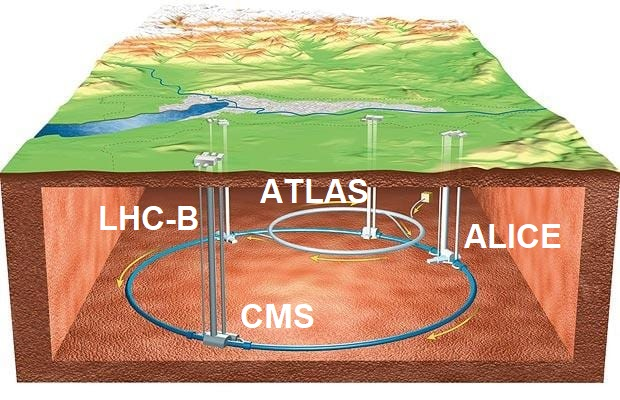
\includegraphics[width=0.6\textwidth]{LHC.jpg}
\end{frame}


\begin{frame}
	\section{Standartinis modelis}
	\frametitle{Standartinis modelis}
	\centering
	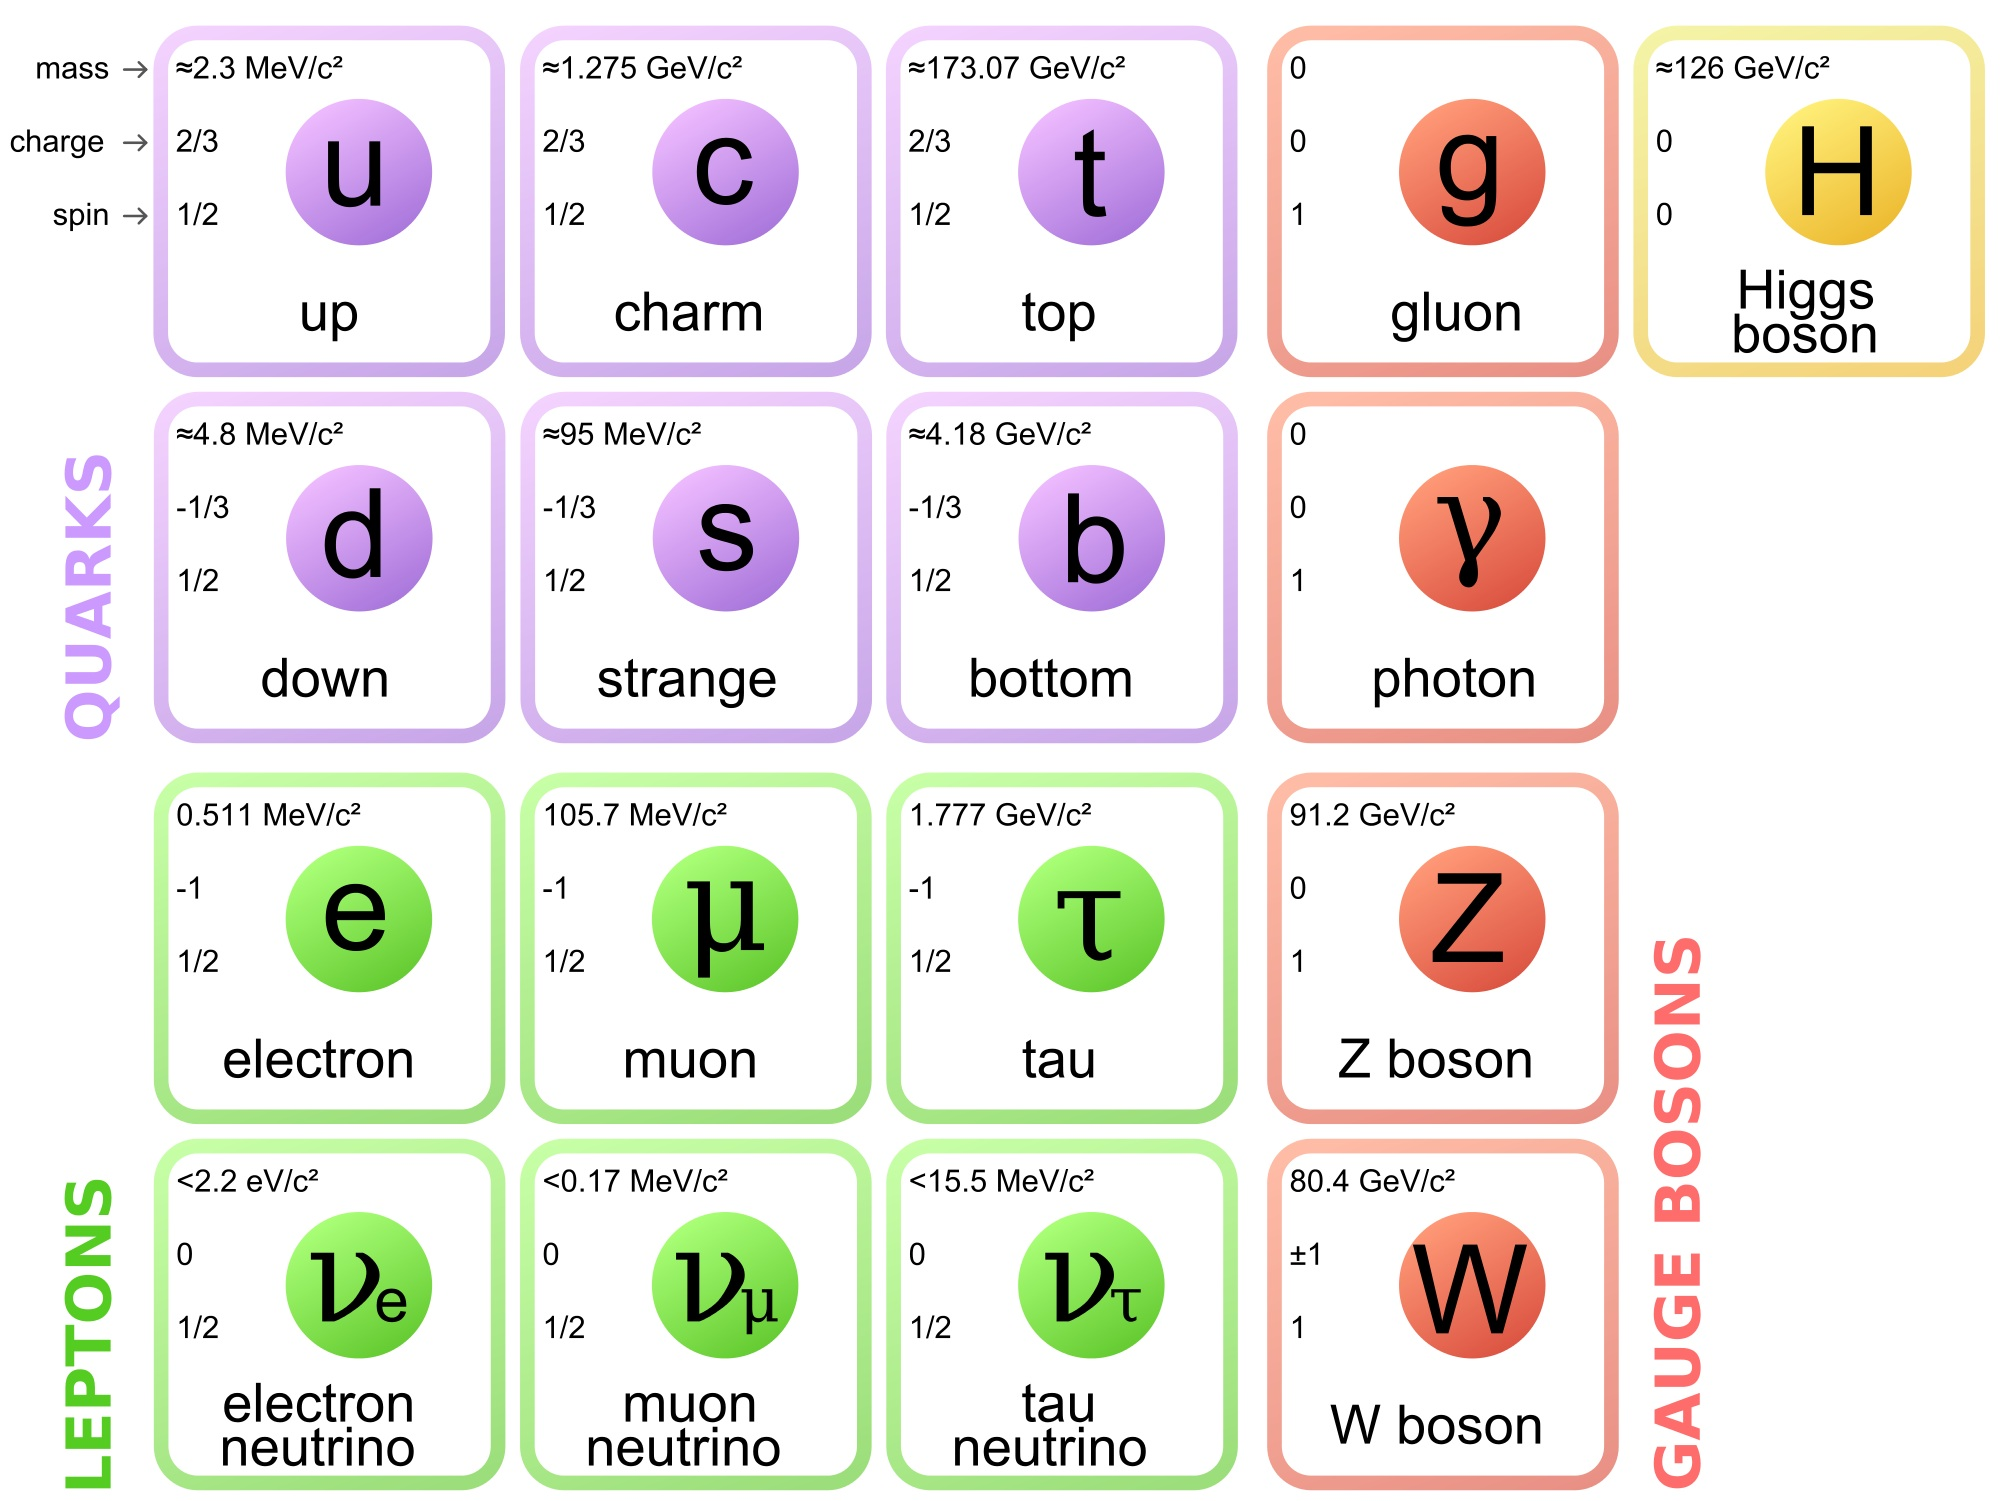
\includegraphics[width=0.8\textwidth]{SM.jpg}
\end{frame}


\begin{frame}
	\section{CMS detektorius}
	\frametitle{Kompaktiškasis miuonų solenoidas}
	\begin{figure}
		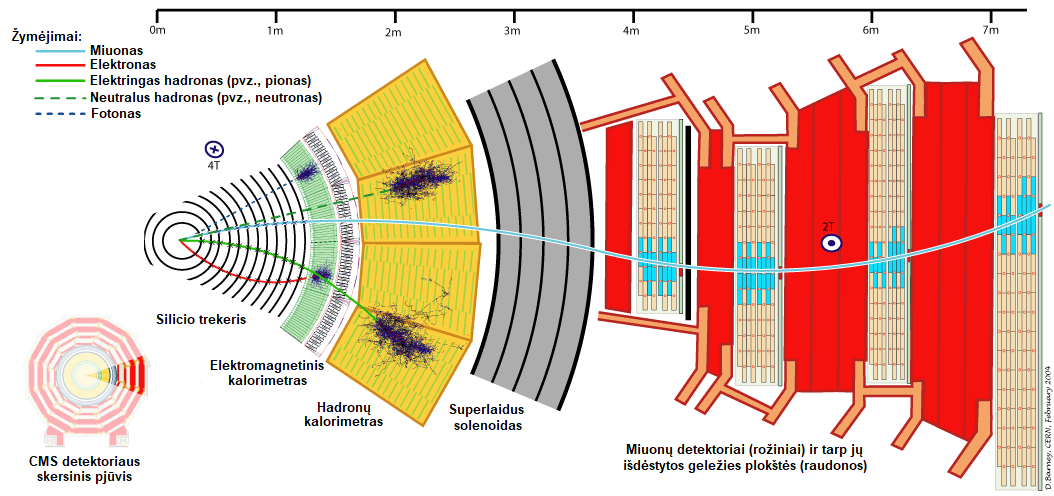
\includegraphics[width=\textwidth]{CMSslice_LT.png}
	\end{figure}
\end{frame}


\begin{frame}
	\section{Drell-Yan procesas}
	\frametitle{Drell-Yan procesas}
	\begin{itemize}
		\item Drell-Yan procesas -- kvarko ir antikvarko anihiliacija, kurios rezultatas -- leptono ir antileptono pora:
		$\mathit{q}\bar{\mathit{q}}\rightarrow \gamma^{*}/\mathit{Z}\rightarrow \mathit{l^{\, +}\! l^{\, -}}$
		($\mathrm{DY}\!\rightarrow\!\mathit{l^{\, +}\! l^{\, -}}$);
		\item Šiame darba nagrinėtos galutinės būsenos -- elektronų bei miuonų poros;
	\end{itemize}
	\begin{minipage}{0.45\textwidth}
		\begin{figure}[H]
			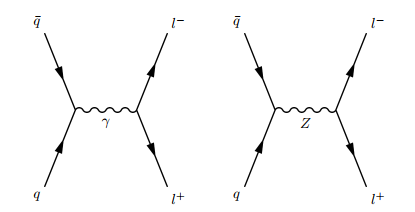
\includegraphics[width=\textwidth]{DYprocess.PNG}
		\end{figure}
		\begin{itemize}
			\item \small Vienas iš matuojamų pasiskirstymų -- diferencialinis reakcijos skerspjūvis
			$\mathrm{d}\sigma/\mathrm{d}\mathit{m}_{\mathit{ll}}$.;
		\end{itemize}
	\end{minipage}
	\hfill
	\begin{minipage}{0.54\textwidth}
		\vspace{-0.2cm}
		\begin{figure}[H]
			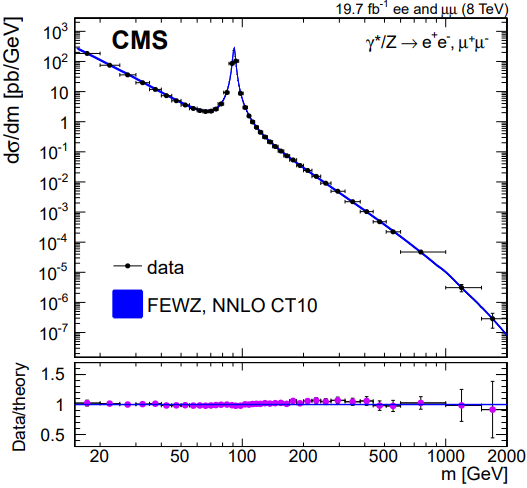
\includegraphics[width=0.8\textwidth]{DYeeCS.PNG}
		\end{figure}
		\vspace{-0.4cm}
		\tiny\centering(CMS Collaboration. Eur.Phys.J. C75 (2015) no.4, 147, 2014.)
	\end{minipage}
\end{frame}


\begin{frame}
	\section{Drell-Yan proceso triukšmai}
	\frametitle{Drell-Yan proceso triukšmai}
	Dalelių detektoriai registruoja ilgai gyvuojančias po protonų susidūrimo susidariusias daleles.

	\medskip

	\begin{itemize}
		% Signalas - mus dominantis procesas
		\item \textbf{Signalas} - mus dominančio proceso galutinė būsena ($\mathrm{DY}\!\rightarrow\!\mathit{e^{+}\! e^{-}}$ arba
		$\mathrm{DY}\!\rightarrow\!\mathit{\mu^{+}\! \mu^{-}}$);
		\item \textbf{Triukšmas} - bet kuris kitas procesas, galintis turėti tokią pačią galutinę būseną, kaip ir signalas;
		\medskip
		\item Pagrindiniai triukšmai:\\
		$\mathit{ZZ}$, $\mathit{tW}$, $\bar{\mathit{t}}\mathit{W}$, $\mathit{WZ}$, $\mathit{WW}$, $\mathit{t}\bar{\mathit{t}}$,
		$\mathrm{DY}\!\rightarrow\!\mathit{\tau^{+\,}\!\tau^{-}}$, $\WJets$, $\mathit{QCD}$;
		\medskip
		\item Triukšmo įvykių skaičiaus įvertinimo būdai:
		\begin{enumerate}
			\item Monte Carlo (MC) modeliavimas;
			\item Matavimu grįsti metodai (pvz., $\emu$ metodas).
		\end{enumerate}
	\end{itemize}
\end{frame}


\begin{frame}
	\section{emu metodo veikimo principas}
	\frametitle{$\emu$ metodo veikimo principas}
	\large $\emu$ metodas leidžia įvertinti indėlį tokių triukšmų, kurių galutinė būsena gali susidėti iš tiek tos pačios,
	tiek skirtingų rūšių leptonų.
	\medskip
	\normalsize
	\begin{itemize}
		%\item Pagrindiniai yra šie triukšmai: $\ZZ$, $\tW$, $\tbarW$, $\WZ$, $\WW$, $\ttbar$, $\DYtau$.
		%\bigskip
		\item Pvz., mus dominančios $\WW\,$ įvykio galutinės būsenos (be skilimo į $\tau$ leptoną):\\[3mm]
		$\WWpm\!\!\rightarrow\!\mathit{e^{+}\!e^{-}}$, $\WWpm\!\!\rightarrow\!\mathit{e^{+}\!\mu^{-}}$,
		$\WWpm\!\!\rightarrow\!\mathit{\mu^{+}\!e^{-}}$, $\WWpm\!\!\rightarrow\!\mu^{+}\!\mu^{-}$;
		\vspace{0.3cm}
		\item Tikėdamiesi, kad $\mathit{N}_{\ee}^{\,\MC}/\mathit{N}_{\emu}^{\,\MC}=\mathit{N}_{\ee}^{\,\Data}/\mathit{N}_{\emu}^{\,\Data}$,
		galime įvertinti $\mathit{N}_{\ee}^{\,\Data}$:
		\begin{equation*}
			\mathit{N}_{\ee}^{\,\mathrm{Įvert.}} = \frac{\mathit{N}_{\ee}^{\,\MC}}{\mathit{N}_{\emu}^{\,\MC}}
												\mathit{N}_{\emu}^{\,\Data} \; .
		\end{equation*}
		Tas pats galioja ir $\mumu$ įvykiams.
	\end{itemize}
\end{frame}


\begin{frame}
	\section{Darbo tikslas}
	\frametitle{Darbo tikslas}
	Šio darbo tikslas:
	\begin{itemize}
		\item Iš didelio duomenų rinkinio išrinkti Drell-Yan proceso įvykius;
		\item Palyginti modeliuotą ir išmatuotą leptonų poros invariantinės masės pasiskirstymus;
		\item $\emu$ metodu įvertinti Drell-Yan proceso triukšmo įvykių skaičių.
	\end{itemize}
	\vspace{0.5cm}
	\small Darbe buvo naudojami $2016$ metais CERN CMS detektoriaus užregistruoti $13 \; \mathrm{TeV}$ energijos
	protonų susidūrimų duomenys, atitinkantys $35.9 \; \mathrm{fb}^{-1}$ integruotąjį šviesį.
\end{frame}


\begin{frame}
	\section{Darbo schema}
	\frametitle{Darbo schema}
	\begin{enumerate}
		\item Įvykių atranka:
		\begin{itemize}
			\item Atranką praėję įvykiai panašūs į Drell-Yan procesą;
		\end{itemize}
		\item Modeliuotų įvykių normavimas ir pataisų pritaikymas:
		\begin{itemize}
			\item Normavimas pagal išmatuotą integruotąjį šviesį;
			\item Pataisos dėl eksperimento ir modeliavimo sąlygų nesutapimo;
		\end{itemize}
		\item Matavimo ir modeliavimo palyginimas;
		\item $\emu$ metodo taikymas triukšmo įvykių įvertinimui.
	\end{enumerate}
\end{frame}

\begin{frame}
	\section{Duomenų ir kodo tvarkymo schema}
	\frametitle{Duomenų ir kodo tvarkymo schema}
	\centering	
	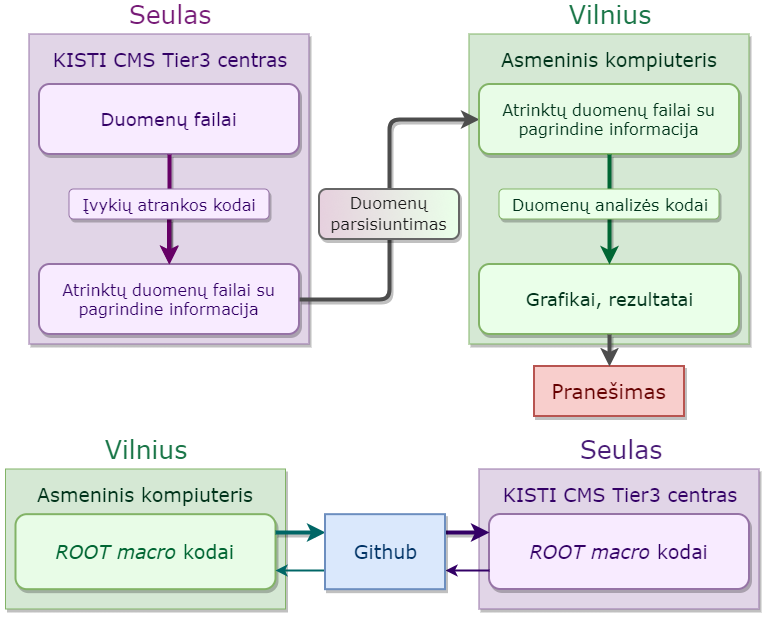
\includegraphics[width=0.8\textwidth]{Duomenu_panaudojimo_schema.png}	
\end{frame}		


\begin{frame}
	\section{Matavimo ir modeliavimo palyginimas}
	\frametitle{Matavimo ir modeliavimo palyginimas}
	\begin{minipage}{0.49\textwidth}
		\centering
		$\ee$
		
		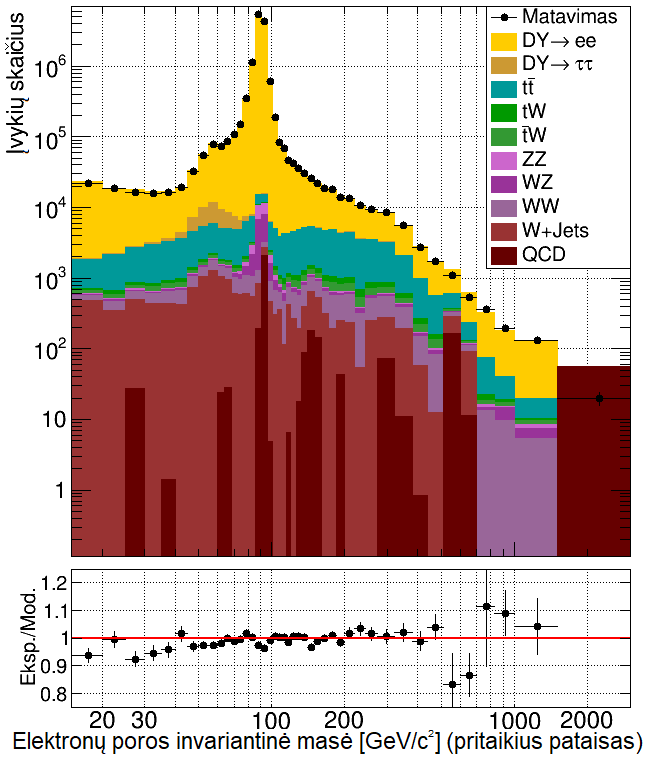
\includegraphics[width=\linewidth]{eeMassAfter_SMALL.png}
	\end{minipage}
	\hfill
	\begin{minipage}{0.49\textwidth}
		\centering
		$\mumu$
		
		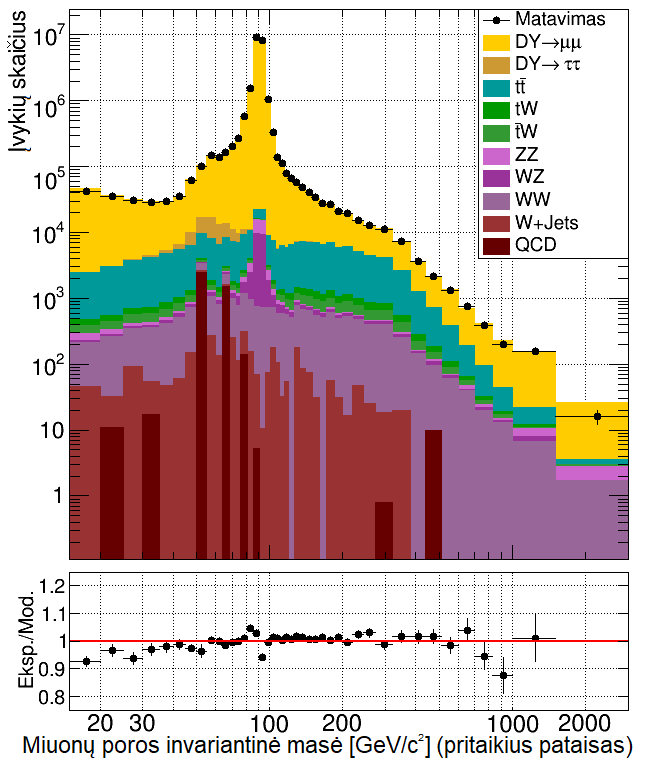
\includegraphics[width=\linewidth]{mumuMassAfter_SMALL.png}
	\end{minipage}
\end{frame}


\begin{frame}
	\frametitle{Pasiruošimas $\emu$ metodo taikymui}
	\vspace{-0.01cm}
	$\emu$ metodas turi savo triukšmą.
	
	\small	
	$\phantom{.}\circ$ Netikrų $\mathit{e}^{\pm}\mu^{\mp}$ įvykių skaičius įvertinamas pasinaudojant $\mathit{e}^{\pm}\mu^{\pm}$ įvykiais\\
	\vspace{0.3cm}
	\begin{minipage}{0.46\textwidth}
		\centering \small
		Prieš netikrų $\emu$ įvykių įvertinimą
		
		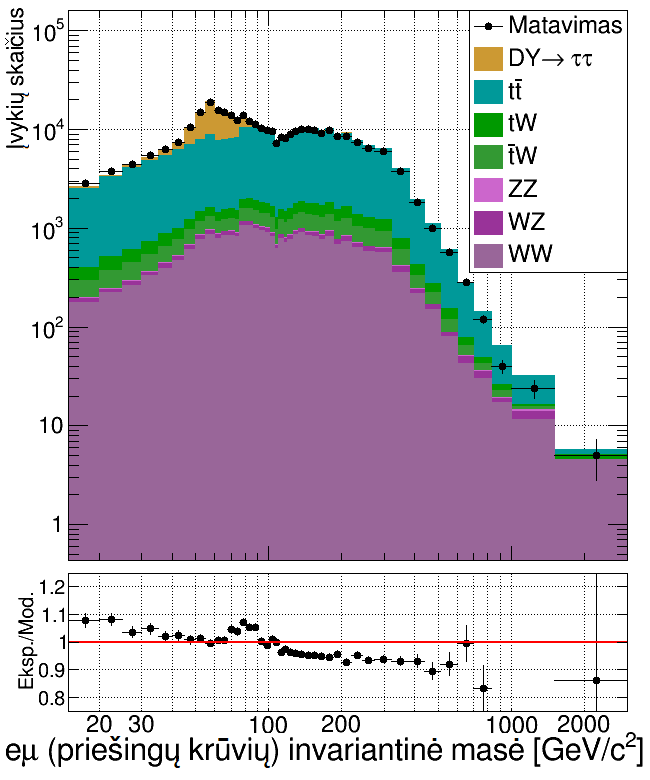
\includegraphics[width=0.9\linewidth]{emuMassOS_SMALL.png}
	\end{minipage}
	\hfill
	\begin{minipage}{0.46\textwidth}
		\centering \small
		Po netikrų $\emu$ įvykių įvertinimo
		
		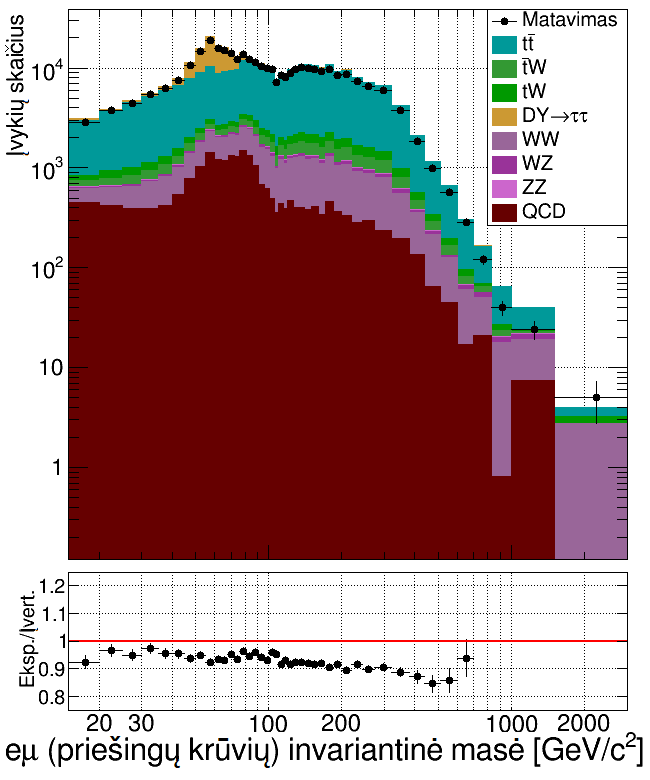
\includegraphics[width=0.9\linewidth]{emuWQCD_SMALL.png}
	\end{minipage}
\end{frame}


\begin{frame}
	\section{$\emu$ metodu įvertinti Drell-Yan triukšmo įvykiai}
	\frametitle{$\emu$ metodu įvertinti Drell-Yan triukšmo įvykiai}
	\begin{minipage}{0.46\textwidth}
		\centering
		$\ee$ 
		
		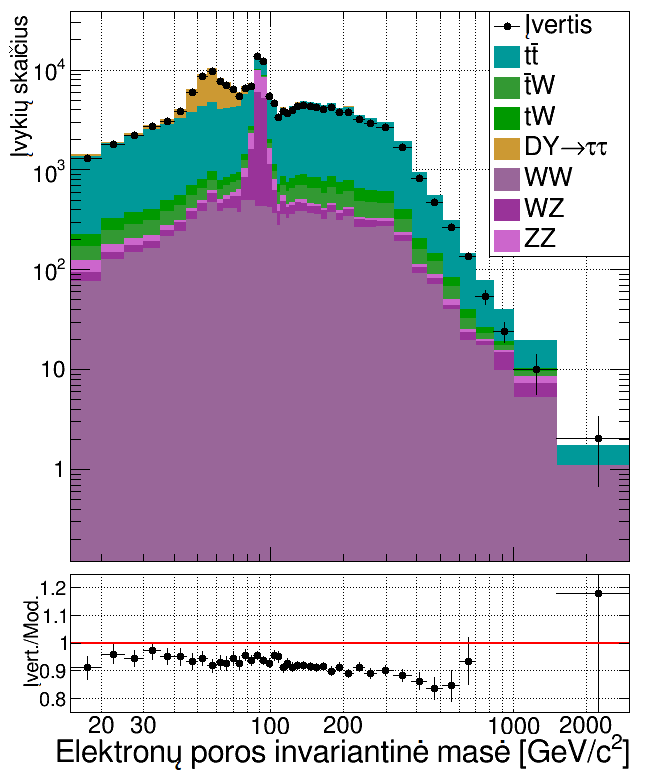
\includegraphics[width=\linewidth]{eeMassEst_SMALL.png}
	\end{minipage}
	\hfill
	\begin{minipage}{0.46\textwidth}
		\centering
		$\mumu$
		
		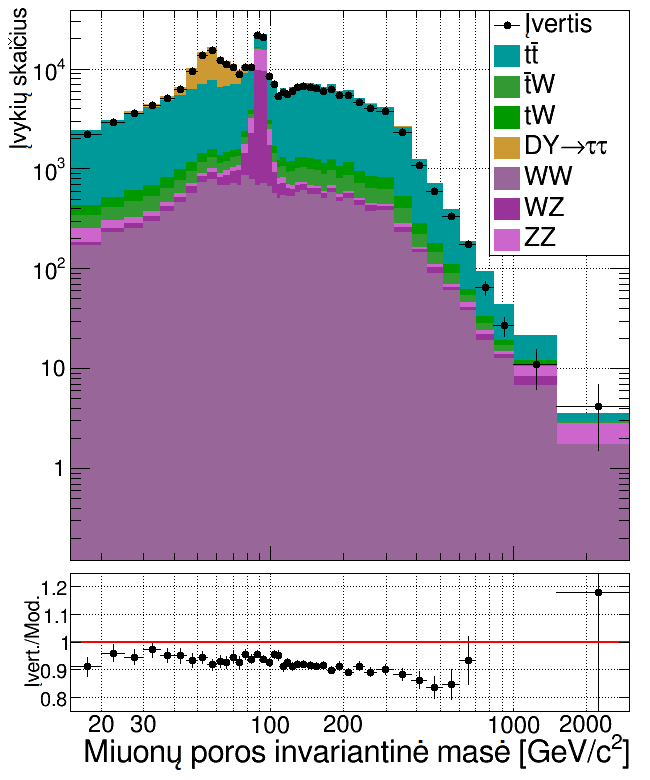
\includegraphics[width=\linewidth]{mumuMassEst_SMALL.png}
	\end{minipage}
\end{frame}


\begin{frame}
	\section{Galutinis rezultatas}
	\frametitle{Išmatuoti invariantinės masės pasiskirstymai}
	Galutinis rezultatas: CMS detektoriaus užregistruotų, modeliuotų, bei $\emu$ metodu įvertintų $\ee$ ir $\mumu$ įvykių
	invariantinių masių pasiskirstymai
	\begin{minipage}{0.49\textwidth}
		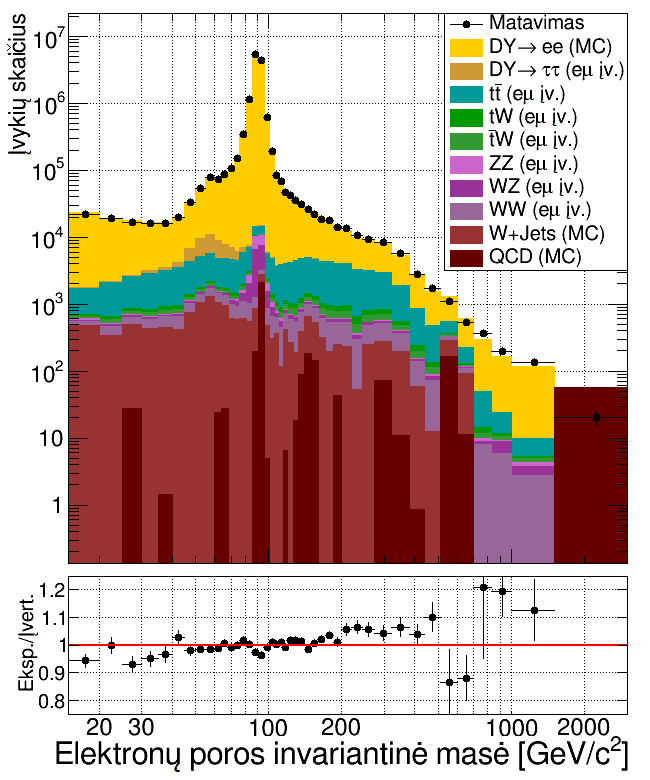
\includegraphics[width=\textwidth]{eeMassFinal_SMALL.png}
	\end{minipage}
	\hfill
	\begin{minipage}{0.49\textwidth}
		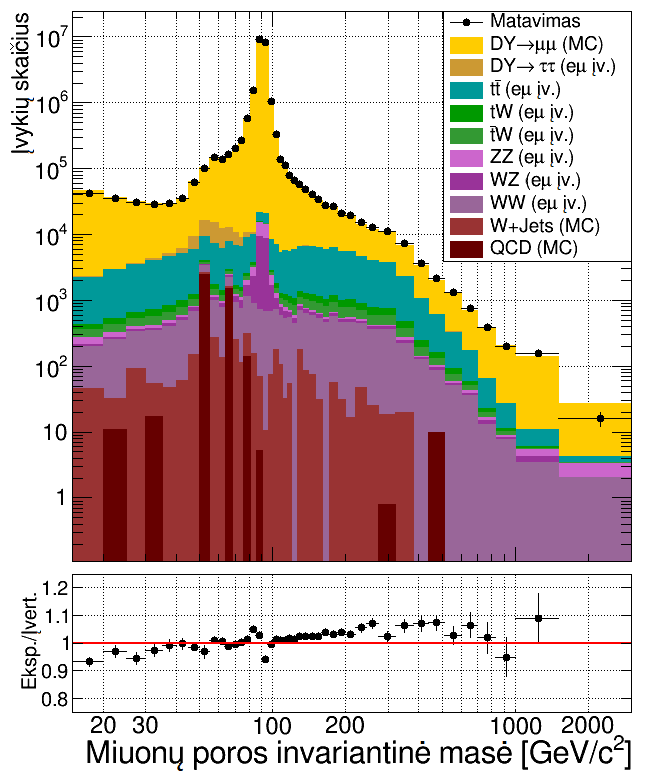
\includegraphics[width=\textwidth]{mumuMassFinal_SMALL.png}
	\end{minipage}
\end{frame}


\begin{frame}
	\section{Išvados}
	\frametitle{Išvados}
	\begin{itemize}
		\item Duomenų rinkinių sukūrimas, saugant tik atranką praėjusius įvykius, gerokai sutrumpina tolimesnės duomenų analizės
		laiką bei supaprastina duomenų saugojimą;
		\smallskip
		\item Eksperimento ir modeliavimo sąlygų nesutapimų pataisos padeda sumažinti atranką praeinančių
		išmatuotų ir modeliuotų įvykių skaičiaus neatitikimus;
		\smallskip
		\item Iš matavimo duomenų įvertinus netikrus $\emu$ įvykius galima geriau įvertinti $\emu$ įvykių skaičių, tačiau pritaikytas
		metodas nepasiteisino ir turi būti peržiūrėtas;
		\smallskip
		\item $\emu$ metodas leidžia įvertinti Drell-Yan proceso triukšmo įvykių skaičių, bet galutinę metodiką dar reikia patobulinti.
	\end{itemize}
\end{frame}

{
\section{Ačiū už dėmesį}
\setbeamercolor{background canvas}{bg=VUdarkred}
\setbeamercolor{palette primary}{bg=VUdarkgray, fg=VUlightgray}
\setbeamercolor{palette secondary}{bg=VUbrightred, fg=VUwhite}
\setbeamercolor{palette tertiary}{bg=VUlightgray, fg=VUdarkgray}
\begin{frame}
	\begin{center}
		\huge \color{VUlightgray}Ačiū už dėmesį
	\end{center}
\end{frame}
}

\appendix

\section{Papildoma informacija}

\begin{frame}
	\subsection{Įvykių skaičių lentelė}
	\frametitle{Galutinių rezultatų lentelė}
	\centering \scriptsize
	\begin{tabular}{|c|c|c|c|}
		\hline
	
	\multirow{2}{7em}{\centering Įvykiai} &
	\multirow{2}{9em}{\centering CMS užregistruoti} &
	\multirow{2}{9em}{\centering Modeliuoti} &
	\multirow{2}{10em}{\centering Įvertinti $e\mu$ metodu} \\
	
 	& & & \\
	\hline \hline
	
	\multirow{2}{7em}{\centering $e\mu$} &
	\multirow{2}{9em}{\centering $(3.110 \pm 0.006) \cdot 10^5$} &
	\multirow{2}{10em}{\centering $(3.359 \pm 0.005) \cdot 10^5$} &
	\multirow{2}{10em}{\centering \textendash }\\
	
 	& & & \\
	\hline
	
	$ee$ ($\WW$, $tW$, &
	\multirow{2}{9em}{\centering\textendash} &
	\multirow{2}{9em}{\centering $(1.883 \pm 0.004) \cdot 10^5$} &
	\multirow{2}{10em}{\centering$\mathbf{(1.749 \pm 0.006) \cdot 10^5}$} \\
	
	$\bar{t}W$, $t\bar{t}$, $\DYtau$) & & & \\
	\hline
	
	\multirow{2}{7em}{\centering $ee$ (visi procesai)} &
	\multirow{2}{9em}{\centering $(1.311 \pm 0) \cdot 10^7$} &
	\multirow{2}{9em}{\centering $(1.344 \pm 0.001) \cdot 10^7$} &
	\multirow{2}{10em}{\centering $\mathbf{(1.343 \pm 0.001) \cdot 10^7}$} \\
	
 	& & & \\
	\hline

	\multirow{2}{7em}{\centering $N_{ee}/N_{ee}^{\mathrm{Obs.}}$} &
	\multirow{2}{9em}{\centering \textendash} &
	\multirow{2}{9em}{\centering $1.0254 \pm 0.0006$} &
	\multirow{2}{10em}{\centering $1.0243 \pm 0.0006$} \\
	
 	& & & \\
	\hline

	$\mumu$ ($\WW$, $tW$, &
	\multirow{2}{9em}{\centering\textendash} &
	\multirow{2}{9em}{\centering $(2.931 \pm 0.005) \cdot 10^5$} &
	\multirow{2}{10em}{\centering$\mathbf{(2.724 \pm 0.009) \cdot 10^5}$} \\
	
	$\bar{t}W$, $t\bar{t}$, $\DYtau$) & & & \\
	\hline
	
	\multirow{2}{7em}{\centering $\mumu$ (visi procesai)} &
	\multirow{2}{9em}{\centering $(2.292 \pm 0) \cdot 10^7$} &
	\multirow{2}{9em}{\centering $(2.315 \pm 0.001) \cdot 10^7$} &
	\multirow{2}{10em}{\centering $\mathbf{(2.313 \pm 0.001) \cdot 10^7}$} \\
	
 	& & & \\
	\hline
	
	\multirow{2}{7em}{\centering $N_{\mumu}/N_{\mumu}^{\mathrm{Obs.}}$} &
	\multirow{2}{9em}{\centering \textendash} &
	\multirow{2}{9em}{\centering $1.0101 \pm 0.0005$} &
	\multirow{2}{10em}{\centering $1.0092 \pm 0.0005$} \\
	
 	& & & \\
	\hline
	\end{tabular}
\end{frame}

\begin{frame}
\subsection{Partonų pasiskirstymo funkcijos}
	\frametitle{Papildoma informacija\\ \small Partonų pasiskirstymo funkcijos}
	\begin{itemize}
		\small
		\item Partonų pasiskirstymo funkcijos aprašo hadronų struktūrą;
		\item Jos reikalingos modeliuojant protonų susidūrimus, skaičiuojant hadronų reakcijų skerspjūvius;
	\end{itemize}
	\centering
	\begin{minipage}{0.49\textwidth}
		\centering
		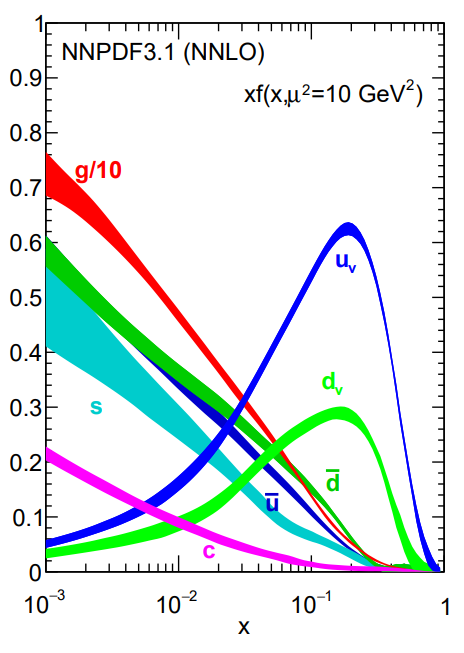
\includegraphics[width=0.62\textwidth]{NNPDF10.PNG}
	\end{minipage}
	\hfill
	\begin{minipage}{0.49\textwidth}
		\centering
		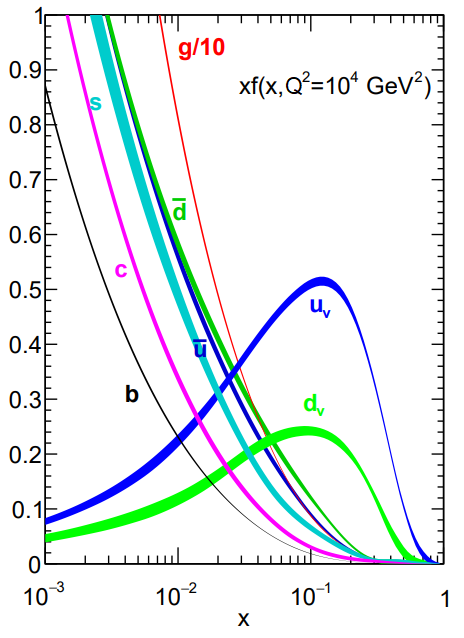
\includegraphics[width=0.62\textwidth]{NNPDF10000.PNG}
	\end{minipage}
	\tiny (The NNPDF Collaboration. Eur.\ Phys.\ J.\ C77 no.\ 10, 663, 2017.)
\end{frame}


\begin{frame}
	\subsection{Invariantinė masė}
	\frametitle{Papildoma informacija\\ \small Invariantinė masė}
	\begin{itemize}
		\item Invariantinė masė -- tai dalelės (rimties) masė, kuri nepriklauso nuo atskaitos sistemos:
		\begin{equation*}
			\mathit{m}_{\, 0}^{\, 2} \mathit{c}^{4} = \mathit{E}^{\, 2}-|\vec{\mathit{p}}|^{2} \mathit{c}^{2} \; ;
		\end{equation*}
		\item Dviejų dalelių invariantinė masė apskaičiuojama taip:
		\begin{equation*}
			\mathit{m}_{\, 12}^{\, 2} \mathit{c}^{4} = ( \mathit{E}_{\, 1}+\mathit{E}_{\, 2} )^{2} -
										   			   | \vec{\mathit{p}_{\, 1}} + \vec{\mathit{p}_{\, 2}} |^{2} \mathit{c}^{2} \; .
		\end{equation*}
	\end{itemize}
\end{frame}

\begin{frame}
	\subsection{Skersinis impulsas, pseudosparta}
	\frametitle{Papildoma informacija\\ \small Skersinis impulsas, pseudosparta}
	\begin{minipage}{0.49\textwidth}
		\begin{itemize}
			\item Detektorius yra išdėstytas cilindriškai aplink protonų spindulį ($\mathit{z}$ ašį);
			\item Matuojamos tik statmenos $\mathit{z}$ ašiai dalelių impulso ir energijos dedamosios --
			$\pT$ ir $\ET$;
			\item Dalelės judėjimo kryptis nusakoma \textit{pseudosparta}:
			\begin{equation*}
				\eta = - \ln \left( \tan \frac{\theta}{2} \right) \; ,
			\end{equation*}
			$\theta$ -- kampas tarp $\mathit{z}$ ašies ir dalelės judėjimo krypties.
		\end{itemize}
	\end{minipage}
	\hfill
	\begin{minipage}{0.48\textwidth}
		\centering
		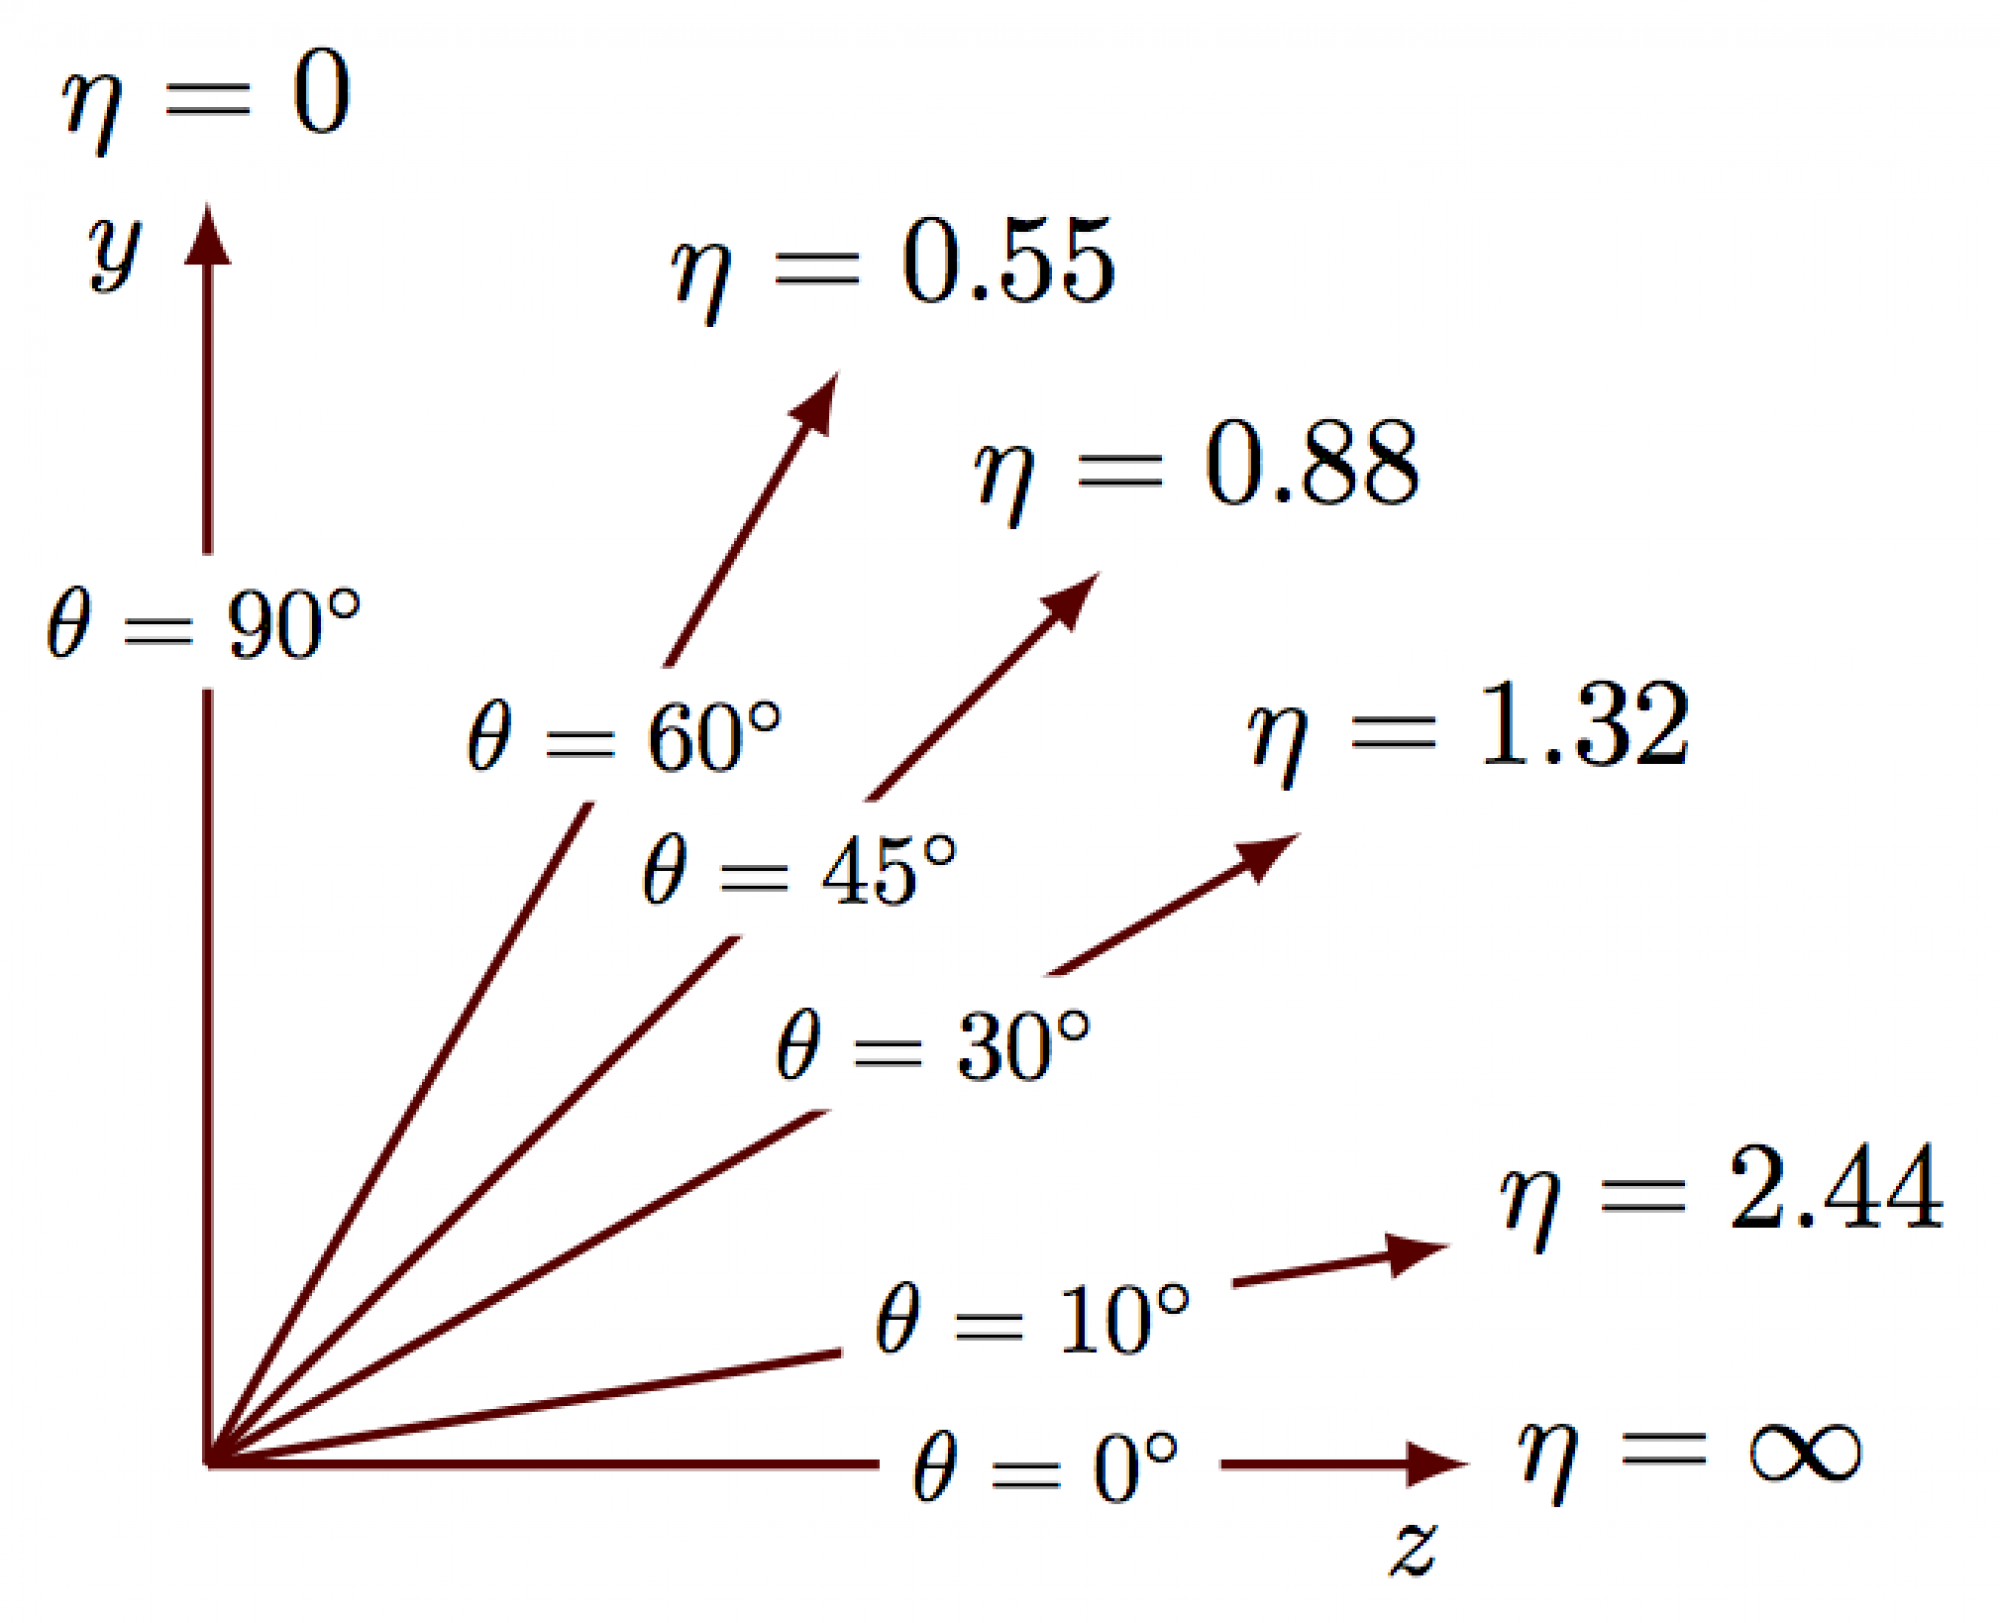
\includegraphics[width=\textwidth]{theta-eta.png}
	\end{minipage}	
\end{frame}

\begin{frame}
	\subsection{Reakcijos skerspjūvis, integruotasis šviesis}
	\frametitle{Papildoma informacija\\ \small Reakcijos skerspjūvis, integruotasis šviesis}
	\begin{itemize}
		\item LHC vykstančių procesų tikėtinumas yra nusakomas reakcijos skerspjūviu $\sigma$, arba
		diferencialiniu reakcijos skerspjūviu $\mathrm{d}\sigma / \mathrm{d}\xi$;
		\item Dalelių skaičius, per laiko vienetą pralekiantis tam tikrą plotą, apibūdinamas šviesiu $\mathcal{L}$;
		\item Norint aprašyti greitintuve vykstančių protonų susidūrimų skaičių naudojamas integruotasis šviesis:
		\begin{equation*}
			\Lumi=\int_{\mathit{t}_1}^{\mathit{t}_2} \mathcal{L}\mathrm{d}\mathit{t} =
			\int_{\mathit{t}_1}^{\mathit{t}_2} \frac{1}{\sigma}\frac{\mathrm{d}\mathit{N}}{\mathrm{d}\mathit{t}} \mathrm{d}\mathit{t} \; ;
		\end{equation*}
		\item Sudauginę integruotąjį šviesį su tam tikro proceso reakcijos skerspjūviu galime įvertinti, kiek kartų
		greitintuve per tam tikrą laikotarpį turėjo įvykti mus dominantis procesas.
	\end{itemize}
\end{frame}

\begin{frame}
	\subsection{Reakcijų skerspjūvių lentelė}
	\frametitle{Papildoma informacija\\ \small Reakcijų skerspjūviai}
	Protonų susidūrimų energija $\sqrt{\mathit{s}}=13$ $\mathrm{TeV}$.
	Integruotasis šviesis $\Lumi=35.9$ \invfb.
	Procesų reakcijų skerspjūviai:
	\begin{table}[H]
		\small
		\begin{tabular}{|c|c|}
			\hline
			Procesas & Reakcijos skerspjūvis (\pb) \\
			\hline\hline
			$\mathrm{DY}\rightarrow \mathit{ll}$ & $24751$ \\
			\hline
			$\ttbar$ & $831.76$ \\
			\hline
			$\tW$ & $35.85$ \\
			\hline
			$\tbarW$ & $35.85$ \\
			\hline
			$\WW$ & $118.7$ \\
			\hline
			$\WZ$ & $47.13$ \\
			\hline
			$\ZZ$ & $16.523$ \\
			\hline
			$\WJets$ & $61526.7$ \\
			\hline
			$\QCD$ ($\mu$) & $1.325 \cdot 10^7$ \\
			\hline
			$\QCD$ ($\mathrm{EM}$) & $1.860 \cdot 10^7$ \\
			\hline
		\end{tabular}
	\end{table}
	\vspace{-0.2cm}
	\small Įvykiai sumodeliuoti su \textsc{aMC@NLO}, \textsc{Powheg}, \textsc{Pythia8} įvykių generatoriais.
\end{frame}

\begin{frame}
	\subsection{Įvykių atranka}
	\frametitle{Papildoma inforamcija\\ \small Įvykių atranka}
	Protonų susidūrimo įvykiai buvo atrenkami vadovaujantis tokiais kriterijais:
	\vspace{-0.2cm}
	\begin{center}
		\footnotesize
		\begin{tabular}{|c|c|}
			\hline
			$\ee$ įvykiai & $\mumu$ įvykiai \\
			\hline\hline
			\multirow{4}{6em}{\centering\textbf{Trigeris:} \ttt{Ele23\_Ele12}} & \textbf{Trigeris:} \\
			& \ttt{HLT\_IsoMu24} arba \ttt{HLT\_IsoTkMu24} \\
			& (bent vienas miuonas turi būti \\
			& tas, kuris aktyvavo trigerį) \\
			\hline
			
			$\mathit{p}_{\mathrm{T}}^{\mathrm{Lead}} > 28 \; \mathrm{GeV}$, &
				\multirow{4}{10em}{\centering$\mathit{p}_{\mathrm{T}}^{\mathrm{Lead}} > 28 \; \mathrm{GeV}$,
				$\mathit{p}_{\mathrm{T}}^{\mathrm{Sublead}} > 17 \; \mathrm{GeV}$,
				$|\eta| < 2.4$} \\
			$\mathit{p}_{\mathrm{T}}^{\mathrm{Sublead}} > 17 \; \mathrm{GeV}$, & \\
			$|\eta_{\mathrm{SC}}| < 2.4$, & \\
			\textbf{išskyrus} $1.4442 < |\eta_{\mathrm{SC}}| < 1.566$ & \\
			\hline
			\textit{Electron MediumID} & \textit{Muon TightID}, $\mathit{I}_{\mathrm{PF}}^{\mathrm{Rel.}} < 0.15$  \\
			\hline
			\multirow{4}{13em}{\centering Visus išvardintus kriterijus turi atitikti lygiai du elektronai} & Du miuonai su mažiausiu bendros \\
			& viršūnės aproksimacijos $\chi^2 < 20$. \\
			& Kampas tarp miuonų trajektorijų \\
			& $\alpha < \pi - 0.005 \; \mathrm{rad}$ \\
			\hline
		\end{tabular}
	\end{center}
	Atrenkant $\emu$ įvykius elektronui buvo taikomi kairiajame, o miuonui -- dešiniajame lentelės stulpelyje aprašyti kriterijai.
\end{frame}

\begin{frame}
	\subsection{Modeliuotų įvykių normavimas}
	\frametitle{Papildoma informacija\\ \small Modeliuotų įvykių normavimas}
	\begin{itemize}
		\item Modeliuotų įvykių skaičius turi būti sunormuotas, kad atitiktų išmatuotą integruotąjį šviesį -- tai daroma įvykiams
		priskiriant svorius;
		\item Jeigu įvykių generatoriaus kiekvienam įvykiui priskirti pradiniai svoriai yra vienodi tada modeliuoto įvykio svorį
		galima apskaičiuoti pagal formulę:
		\begin{equation*}
			\omega = \frac{\sigma \Lumi}{\mathit{N}} \; ;
		\end{equation*}
		\item Bendru atveju (ir šiuo atveju):
		\begin{equation*}
			\omega_{\mathit{i}} = \omega_{\mathit{i}}^{\mathrm{gen}}
								  \frac{\sigma \Lumi}{\sum_{\mathit{j}=1}^{\mathit{N}}\omega_{\mathit{j}}} \; .
		\end{equation*}
	\end{itemize}
\end{frame}


\begin{frame}
	\subsection{Pataisų taikymas}
	\frametitle{Papildoma informacija\\ \small Pataisų taikymas I}
	Tarp eksperimento ir modeliavimo nesutapo šios sąlygos:
	\begin{itemize}
		\item Protonų susidūrimų skaičiaus tikimybė;
		\item Elektronų energijos bei miuonų skersinio impulso matavimo skalės;
		\item Trigerių suveikimo efektyvumai;
		\item Leptonų atpažinimo ir jų trajektorijų atkūrimo efektyvumai;
		\item Miuonų trajektorijos atskirumo įvertinimo efektyvumas.
	\end{itemize}
	Į šiuos neatitikimus buvo bandoma atsižvelgti taikant pataisas -- koreguojant elektronų energijos ir miuonų impulso vertes,
	bei priskiriant papildomus svorius modeliuotiems įvykiams.
\end{frame}

\begin{frame}
	\frametitle{Papildoma informacija\\ \small Pataisų taikymas II}
	Atrinktuose $\ee$ įvykiuose atkurtų pirminių viršūnių skaičiaus paiskirstymai prieš ir po pataisos pagal protonų susidūrimų
	tankį pritaikymo:
	\begin{minipage}{0.49\textwidth}
		\centering
		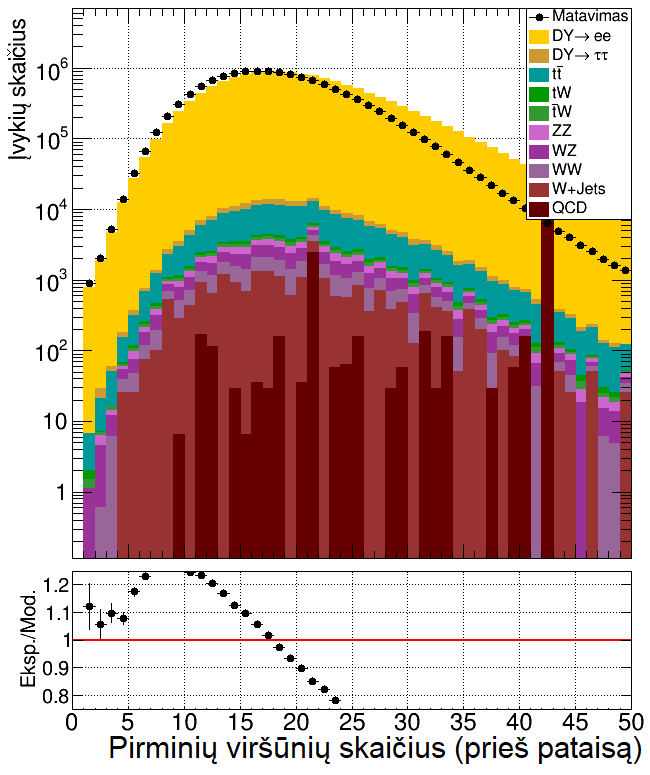
\includegraphics[width=0.9\textwidth]{eeNVTXbefore_SMALL.png}
	\end{minipage}
	\hfill
	\begin{minipage}{0.49\textwidth}
		\centering
		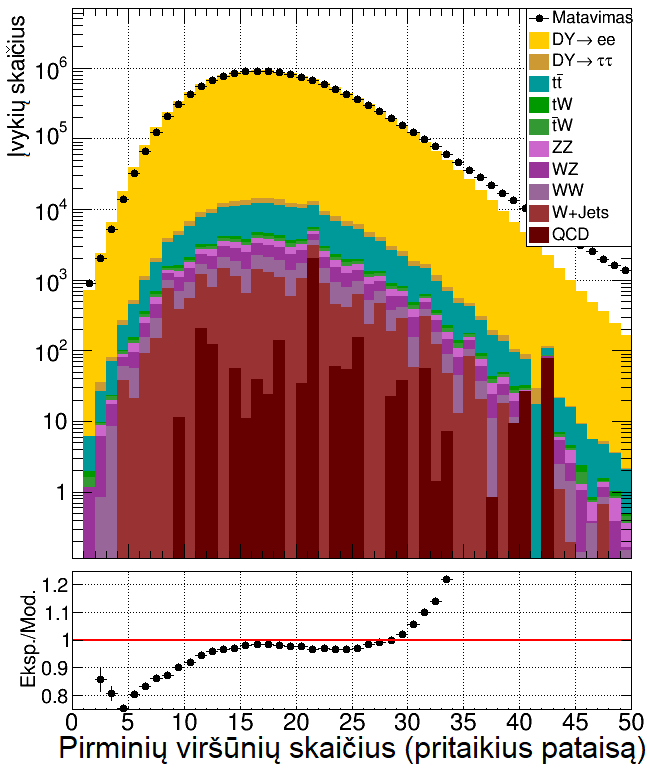
\includegraphics[width=0.9\textwidth]{eeNVTXafter_SMALL.png}
	\end{minipage}
\end{frame}

\begin{frame}
	\subsection{ee pataisų taikymas}
	\frametitle{Papildoma informacija\\ \small Pataisų taikymas III}
	CMS detektoriaus užregistruotas ir modeliuotas $\ee$ invariantinės masės pasiskirstymai prieš ir po pataisų pritaikymo:
	\begin{minipage}{0.49\textwidth}
		\centering
		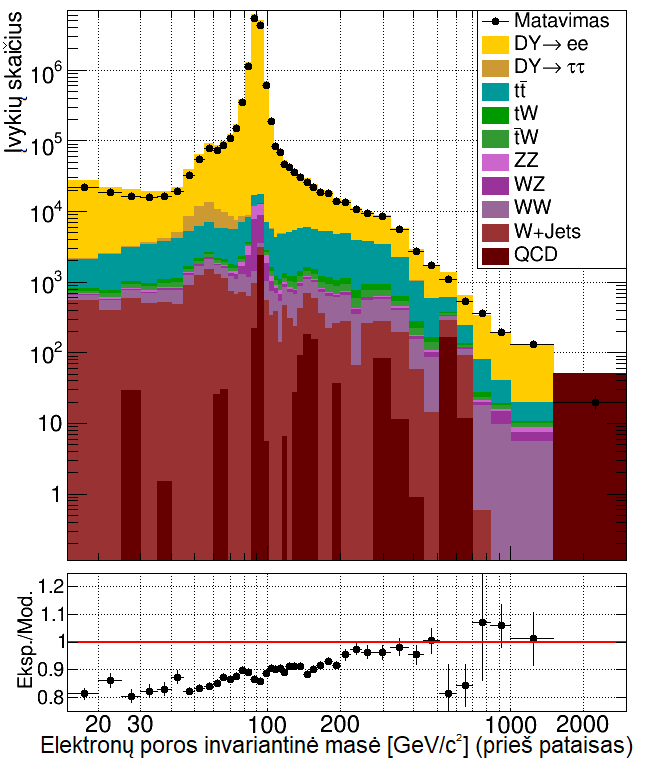
\includegraphics[width=0.9\linewidth]{eeMassBefore_SMALL.png}
	\end{minipage}
	\hfill
	\begin{minipage}{0.49\textwidth}
		\centering
		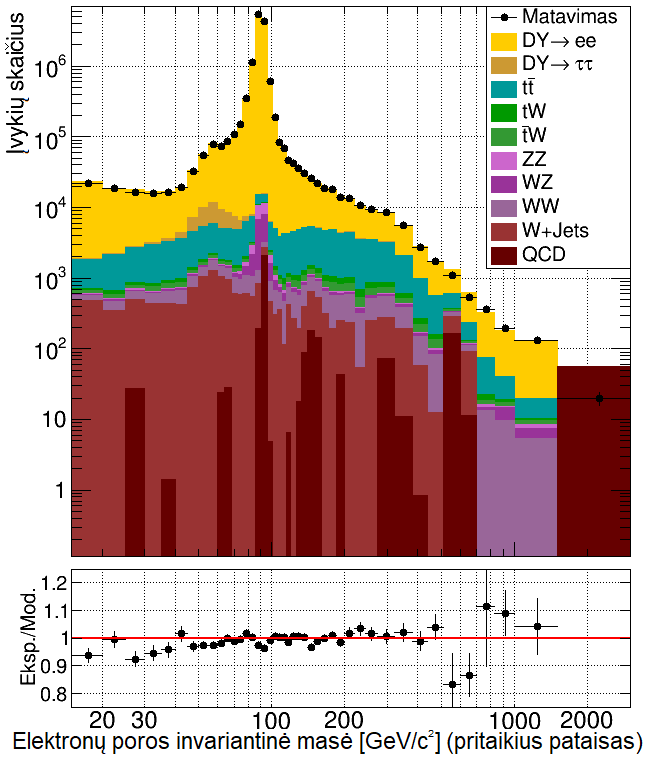
\includegraphics[width=0.9\linewidth]{eeMassAfter_SMALL.png}
	\end{minipage}
\end{frame}

\begin{frame}
	\subsection{mumu pataisų taikymas}
	\frametitle{Papildoma informacija\\ \small Pataisų taikymas IV}
	CMS detektoriaus užregistruotas ir modeliuotas $\mumu$ invariantinės masės pasiskirstymai prieš ir po pataisų pritaikymo:
	\begin{minipage}{0.49\textwidth}
		\centering
		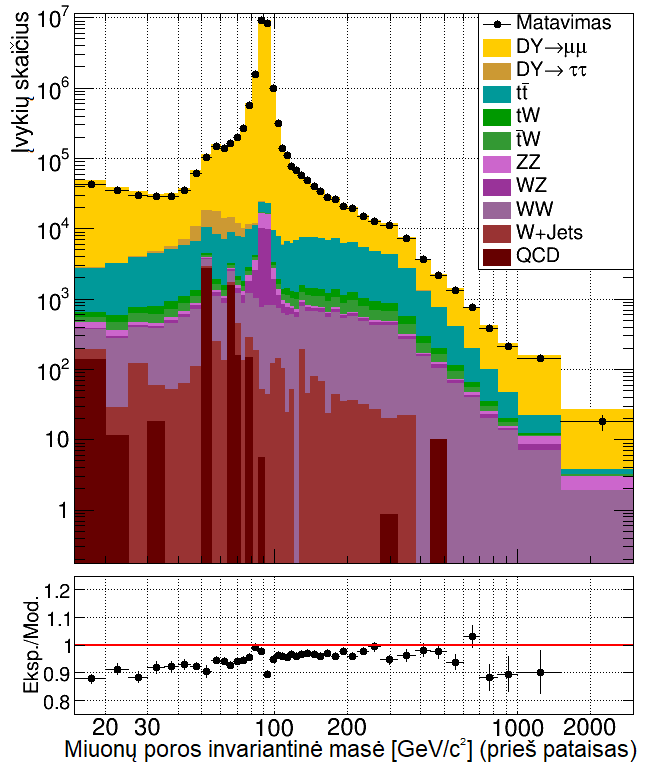
\includegraphics[width=0.9\linewidth]{mumuMassBefore_SMALL.png}
	\end{minipage}
	\hfill
	\begin{minipage}{0.49\textwidth}
		\centering
		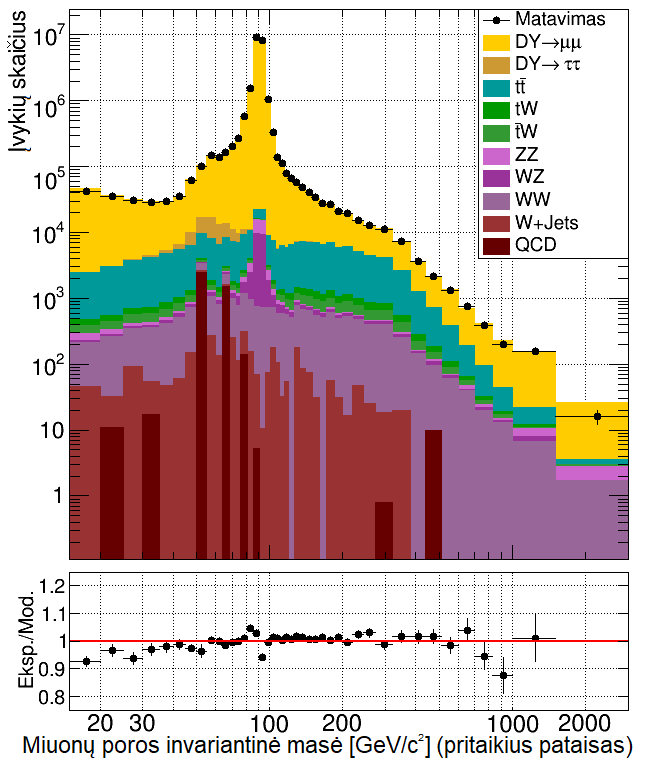
\includegraphics[width=0.9\linewidth]{mumuMassAfter_SMALL.png}
	\end{minipage}
\end{frame}

\begin{frame}
	\subsection{Efektyvumų matrica}
	\frametitle{Papildoma informacija\\ \small Pataisų taikymas V}
	Efektyvumų pataisų svoriai modeliuotiems įvykiams buvo gaunami lyginant eksperimentinių ir modeliuotų efektyvumų matricas:\\
	\vspace{0.1cm}
	\centering
	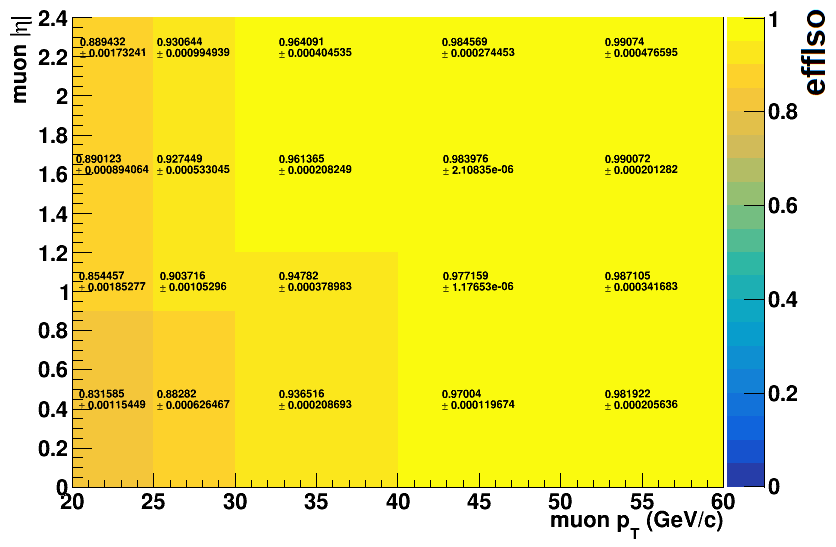
\includegraphics[width=0.8\textwidth]{efficiency.png}
\end{frame}

\begin{frame}
	\subsection{Matavimu grįsti triukšmo įvykių įvertinimo metodai}
	\frametitle{Papildoma informacija\\ \small Matavimu grįsti triukšmo įvykių įvertinimo metodai}
	\textbf{Kontrolinėje srityje}, kurioje dominuoja triukšmo įvykiai apskaičiuotas įvykių skaičius transformuojamas į triukšmo
	įvykių skaičių \textbf{signalo srityje}.\\
	\vspace{0.3cm}
	Pagrindiniai matavimu grįsti triukšmo įvykių skaičiaus įvertinimo metodai:
	\begin{itemize}
		\item Klaidingo atpažinimo metodas\\
			Skirtas įvertinti procesams, kuriuose gali susidaryti čiurkšlės (angl.\ \textit{jets});
		\item ABCD metodas\\
			Skirtas įvertinti procesams, kuriuose gali susidaryti čiurkšlės;
		\begin{block}{$\emu$ metodas}
			Skirtas įvertinti procesams, kuriuose susidaro dvi nestabilios dalelės, skylančios į leptonus nepriklausomai;
		\end{block}
		\item Ir kt.
	\end{itemize}
\end{frame}

\begin{frame}
	\subsection{Triukšmų įskaitymas}
	\frametitle{Papildoma informacija\\ \small Netikrų $\emu$ įvykių įskaitymas taikant $\emu$ metodą I}
	\begin{equation*}
		\mathit{N_{ee}^{\,\mathrm{Įvert.}}} = \frac{\mathit{N}_{\ee}^{\,\mathrm{MC}}}{\mathit{N}_{\emu}^{\,\mathrm{MC}}}
											\mathit{N}_{\emu}^{\,\mathrm{Data}} \; ;
	\end{equation*}
	\begin{itemize}
		\item Problema: tarp atrinktų $\emu$ įvykių yra ir netikrų $\emu$ įvykių;
		\item Šių \quotedblbase{}$\emu$ triukšmo\textquotedblleft{} įvykių skaičių buvo bandoma įvertinti iš matavimo, atsirenkant tokius įvykius,
		kuriuose užregistruotas elektronas ir miuonas yra vienodo elektrinio krūvio;
		\item Skirtumas tarp eksperimento metu užregistruoto ir modeliuoto tikrų vienodo krūvio elektrono ir miuono
		invariantinės masės pasiskirstymų laikomas netikrų ($\QCD$) elektrono ir miuono invariantinės masės pasiskirstymu:
		\begin{equation*}
			\mathit{N}_{\emu \, \mathrm{SS}}^{\,\QCD} = \mathit{N}_{\emu \, \mathrm{SS}}^{\,\Data} -
													  \mathit{N}_{\emu \, \mathrm{SS}}^{\,\MC \, (\ttbar + \tW + \tbarW + \WW + \WZ + \ZZ + \DYtau)} \; ;
		\end{equation*}
	\end{itemize}
\end{frame}


\begin{frame}
	\section{Triukšmų įskaitymas}
	\frametitle{Papildoma informacija\\ \small Netikrų $\emu$ įvykių įskaitymas taikant $\emu$ metodą II}
	\begin{minipage}{0.44\textwidth}
		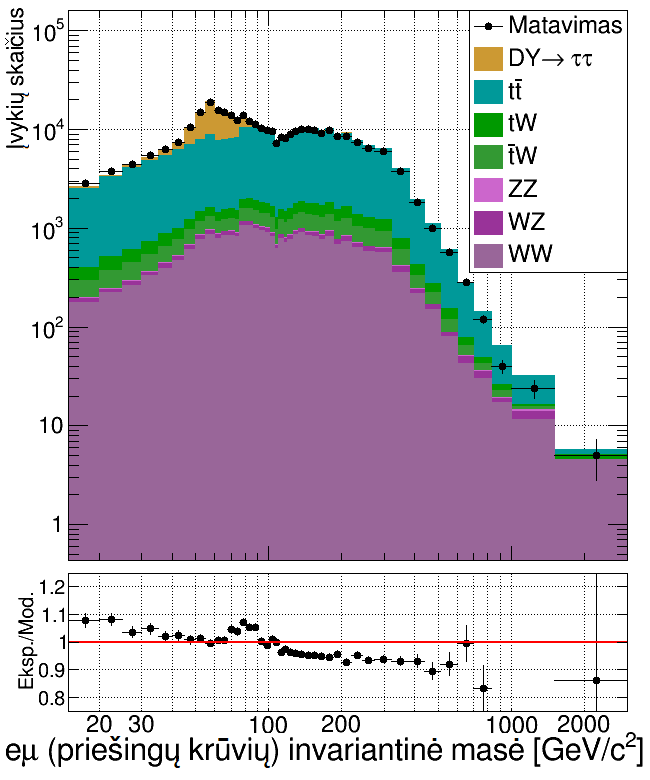
\includegraphics[width=\linewidth]{emuMassOS_SMALL.png}
	\end{minipage}
	\hfill
	\begin{minipage}{0.44\textwidth}
		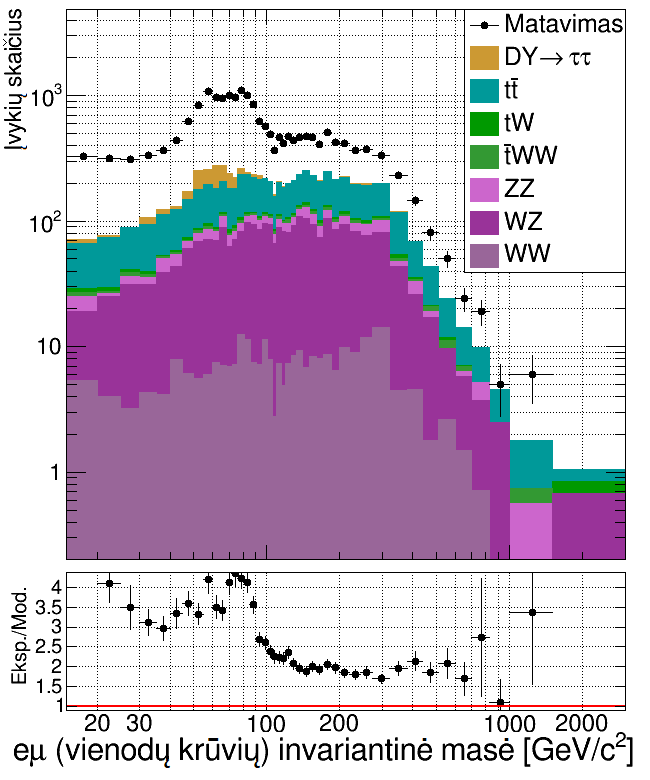
\includegraphics[width=\linewidth]{emuMassSS_SMALL.png}
	\end{minipage}
\end{frame}


\begin{frame}
	\frametitle{Papildoma informacija\\ \small Netikrų $\emu$ įvykių įskaitymas taikant $\emu$ metodą III}
	\begin{itemize}
		\item Gautasis įvykių skaičius transformuojamas į netikrų priešingo krūvio $\emu$ įvykių skaičių, panaudojant teoriškai apskaičiuojamą
		daugiklį $\mathit{R} \approx 0.5715$:
		\begin{equation*}
			\mathit{N}_{\emu \, \mathrm{OS}}^{\,\QCD} = \frac{\mathit{N}_{\emu \, \mathrm{SS}}^{\,\QCD}}{\mathit{R}} \; .
		\end{equation*}
	\end{itemize}
	\centering
	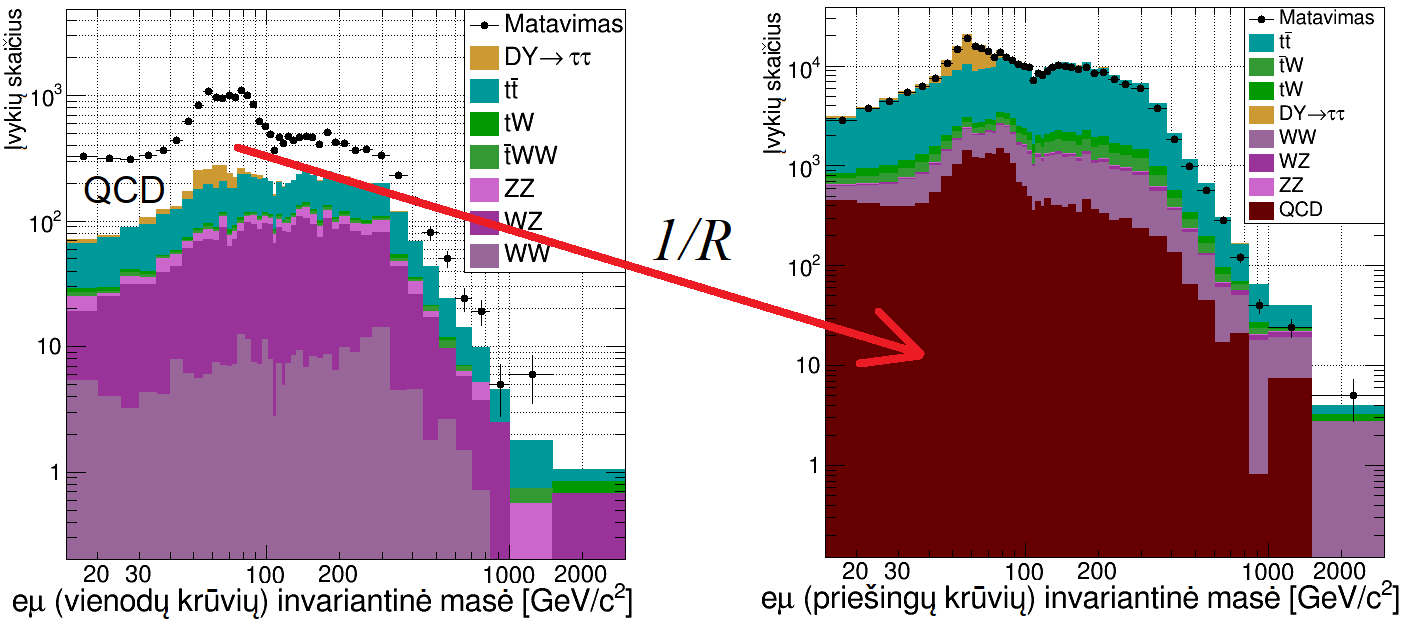
\includegraphics[width=0.9\textwidth]{emuMassSStoOS.png}
\end{frame}

\begin{frame}
	\subsection{Neapibrėžtumų įvertinimas}
	\frametitle{Papildoma informacija\\ \small Neapibrėžtumų įvertinimas}
	\begin{itemize}
		\item CERN LHC vykstantys protonų susidūrimo įvykiai yra Puasono įvykiai;
		\item CMS detektoriaus užregistruotų įvykių skaičiaus statistinis neapibrėžtumas skaičiuojami kaip kvadratinė šaknis iš įvykių skaičiaus:
		\begin{equation*}
			\Delta \mathit{N}_\mathrm{Data} = \sqrt{\mathit{N}_\mathrm{Data}} \; ;
		\end{equation*}
		\item Modeliuotų įvykių skaičiaus statistinis neapibrėžtumas skaičiuojamas kaip kvadratinė šaknis iš modeliuotų įvykių svorių kvadratų sumos:
		\begin{equation*}
			\Delta \mathit{N}_\mathrm{MC} = \sqrt{\sum_{\mathit{i}=1}^{\mathit{n}}\mathit{w_{i}}^{2}} \; .
		\end{equation*}
	\end{itemize}
\end{frame}

\end{document}
